% Geometry, font
\documentclass[12pt, letter]{article}
\usepackage[margin=0.8in]{geometry}
\usepackage[T1]{fontenc}
\usepackage{fourier}
\usepackage{titling}
\setlength{\droptitle}{-5em} 
\usepackage[parfill]{parskip}
\usepackage{graphicx}
\usepackage{hyperref}

% Math stuff
\usepackage{amssymb}
\usepackage{bm}

% Code Highlighting
\usepackage{minted}
\usemintedstyle{solarizedlight}

\author{Zach Neveu}
\title{ Day 5 Notes }

\begin{document}
\maketitle

\section{Agenda}%
\label{sec:agenda}
\begin{itemize}
	\item Review of NPC
	\item Proving problems NP Complete
	\item Examples
	\item Subproblems
\end{itemize}

\section{Announcements}%
\label{sec:announcements}
\begin{itemize}
	\item Quiz on Wednesday - through most recent homework (NOT NPC)
	\begin{itemize}
		\item Know big ideas
		\item Know important terms
		\item Know practical applications
		\item Re-Solve problems we've seen for practice
		\item Make sure we've done the reading
		\item No code on quiz
	\end{itemize}
	\item Finish up reading about NPC stuff
\end{itemize}

\section{NP Completeness Review}%
\label{sec:np_completeness_review}

\subsection*{To be in NP a problem, $L$, must:}
\begin{itemize}
	\item $L \in NP$
	\item For every problem $L' \in NP$, $L' \le L$
\end{itemize}

\subsection*{How to Prove}
\begin{itemize}
	\item Prove that $SAT \le L$
	\item Given a problem $\pi \in NP$ whos complexity is unknown, how to find?
	\item Define special case $\pi'$ containing a subset of the instances of  $\pi$ 
	\item Prove that $\pi'$ is NPC
	\item $\pi' \le \pi$ because every special case is already a regular case as well
	\item $\pi$ is NPC, since its simpler subset, $\pi'$ is NPC
	\item QUIZ: Explain why the last bullet is true
\end{itemize}


\section{Examples}%
\label{sec:examples}
Partition: given a set \textbf{A} and size $s(\bm{A})$ for all $a \in \bm{A}$ is there a subset $\bm{A'} \in \bm{A}$ such that $\sum s(a) = \sum s(!a)$ where  $!a$ is the set of elements not in s. Basically, divide $A$ into two sets with equal size. \\

Knapsack: given a set, $U$, a size $s(u)$ and a value  $v(u)$ for all $u \in U$, and size constraint  $B$, and a value goal $K$, is there a subset $u'\in U$ such that $\sum s(u') \le B$ and $\sum v(u') \ge K$? \\

\begin{itemize}
 \item Claim: Partition $\le$ Knapsack
 \item Prove: Given an instance of Partition, show that we can produce an instance of knapsack with the same answer.
 \item Answer: Set $K=B=\frac{1}{2}\sum s(u)$.
 \item Idea: sandwich K & B such that knapsack will find same answer as partition
 \item If Knapsack is yes instance, Partition will be yes instance
 \item If Partition is yes instance, Knapsack is yes instance
 \item If partition is NPC, Knapsack is NPC
\end{itemize}

\section{Problem as Tuple}%
\label{sec:problem_as_tuple}
\begin{itemize}
	\item Consider a problem $\pi = (D,Y)$ where D is all instances, Y is all yes instances
	\item Sub-problem $\pi' = (D',Y')$ reduces to $\pi$
\end{itemize}
\begin{figure}[h]
	\centering
	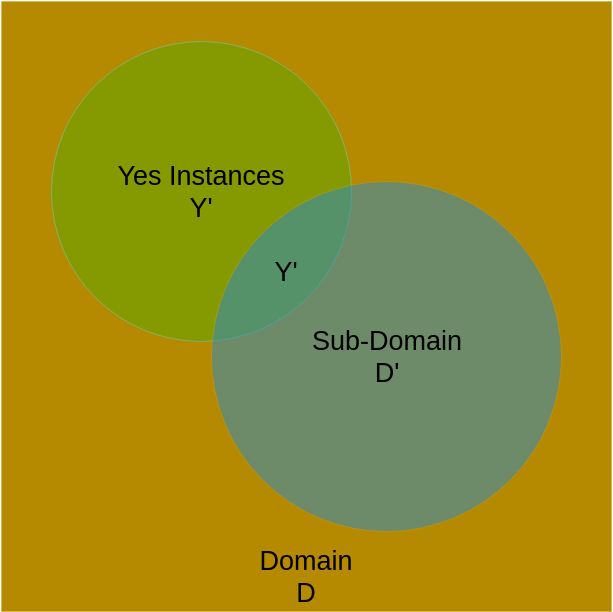
\includegraphics[width=0.8\textwidth]{imgs/domain}
	\caption{Relation of D, D', Y, Y'}
	\label{fig:domain}
\end{figure}

\end{document}
